\section{Evaluating a context policy}
\label{sec:row-4}

Two summaries of the same history led the agent to different decisions, so we measure a policy by the decisions it supports and by what it costs, stress it with the commitments the run depends on, and close with next week.

\subsection{An evaluation measures quality and total work}
\label{sec:it-10-1}

\bi
\item \textbf{Task success:} the agent makes the right next vending decision.
\item \textbf{Evidence:} the facts, conditions and sources the decision needs survive.
\item \textbf{Faithfulness:} nothing is added or changed, and nothing open is settled.
\item \textbf{Cost:} the token ratio with its convention, and every call, fetch and charge.
\ei

The course combines these measures. Task success checks the next vending decision. Evidence checks the facts, conditions and source references that the decision needs. Faithfulness checks for unsupported claims, changed meaning, and uncertainty that becomes a settled claim. Compression compares the original and replacement token counts under a stated ratio convention. Total work counts summary calls, retrieval, later model calls, elapsed time and charges. The last two share the slide's Cost bullet.

LLMLingua-2 reports task scores, compression and latency together. Include the uncompressed input and a simple selection baseline, compare equal input budgets where possible, and report the uncertainty across repeated runs. A compression ratio alone cannot show that a policy serves its task. These five measures cover the three objectives of the slide \hyperref[sec:it-5-1]{``Context supplies each call within a budget.''} and its cost.

The rubric is the course's, and no paper reports results for it. The ``60k to 40 tokens'' of the compression check reuses the abstractive figure's illustrative counts, so we state the ratio convention with it, for example original over replacement, 1500 to 1.

\begin{figure}[htbp]
\centering
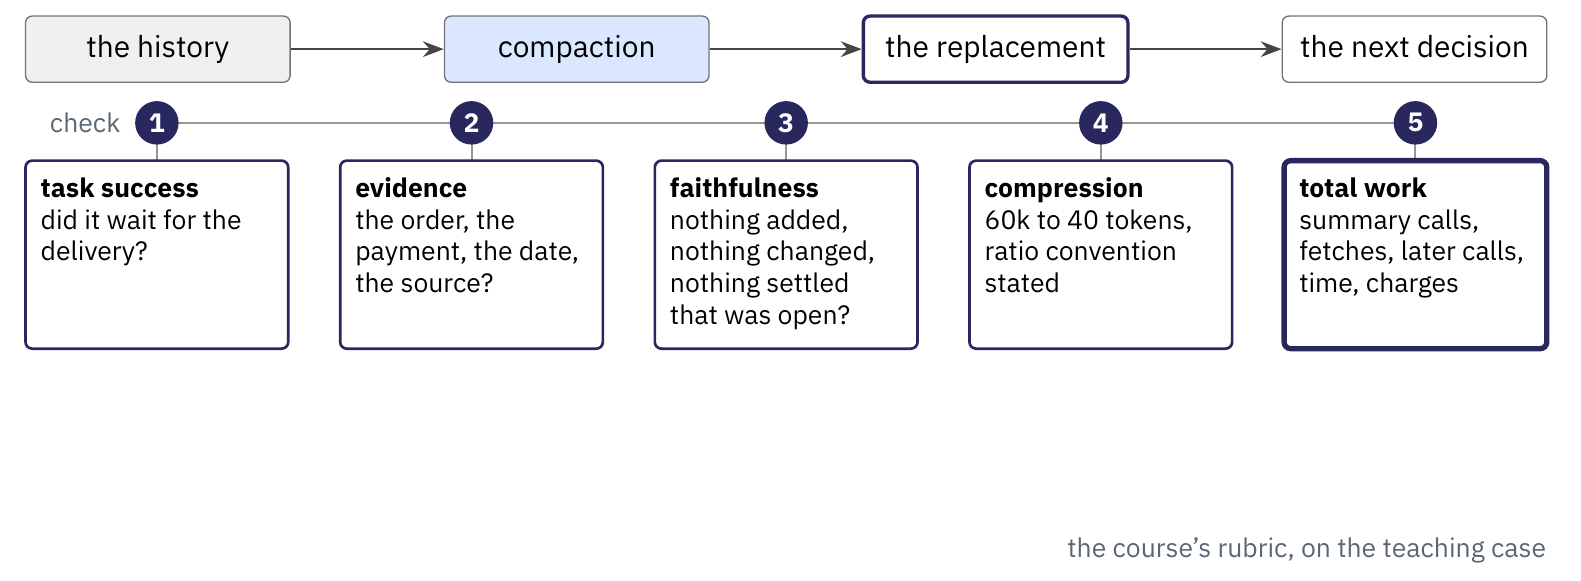
\includegraphics[width=\linewidth]{context/evaluation-5.png}
\caption{An evaluation measures quality and total work. The figure as it stands after the build's last click.}
\label{fig:evaluation-5}
\end{figure}

\paragraph{The figure, stage by stage.}
\be
\item The run lane: compaction turns the history into the replacement, and the next decision is made from the replacement. Check 1, task success, asks of the vending run: did it wait for the delivery?
\item Check 2, evidence: the order, the payment, the date, the source? The replacement must still carry each fact the next decision needs.
\item Check 3, faithfulness: nothing added, nothing changed, nothing settled that was open? Whether the delivery has arrived is still open, and the replacement must keep it open.
\item Check 4, compression: 60k to 40 tokens, ratio convention stated. The counts are those of the abstractive summary that leaves out the paid order, and the report states which way the ratio runs.
\item Check 5, total work: summary calls, fetches, later calls, time, charges. The five checks are reported together, because a compression ratio alone cannot show that a policy serves its task.
\ee

\begin{takeaway}A policy is judged by the decisions it supports and by the work it costs.\end{takeaway}

\subsection{Stress tests target what compaction can lose}
\label{sec:it-10-2}

\bi
\item \textbf{Delayed effects:} a delivery due after the next compaction must stay recorded.
\item \textbf{Recurring obligations:} the daily fee must survive repeated compaction.
\item \textbf{Updates and provenance:} a revised delivery date must carry its source.
\item \textbf{Repeated compaction:} the open order must survive several replacements.
\ei

Each stress test reuses the test logic of RULER and of Lost in the Middle. RULER plants facts with known answers in synthetic text, fixes the task, changes only the input length, scores every answer automatically and grades each length against a fixed bar. Lost in the Middle moves the evidence to chosen positions. A stress test plants a commitment in the run's history, compacts, and checks automatically that the next decision still has it. We vary what the two papers vary: the commitment sits early, in the middle or late in the history, and the history grows to each length the run reaches before it compacts. Two of the drawn tests exercise operations that RULER grades separately (the backup slide \hyperref[sec:it-B-6-3]{``Effective length depends on the operation.''}): the daily fee is one fact to find, and a revised delivery date is a chain to trace to its source. None of the four aggregates, and a full suite adds one, such as the units still on order. The course proposes these application tests, and neither paper reports results for them. The fourth test has published evidence behind it: Agentic Context Engineering (Zhang et al., ICLR 2026) describes context collapse, in which iterative rewriting erodes details over time.

For the vending run, we test an empty shelf while an order remains in transit, a second order before the first arrives, and a delivery notice that changes the expected date. Source access is verified separately from the summary's wording.

The four drawn tests are the course's. Neither the figure nor the bullets show a position or a length test.

\begin{figure}[htbp]
\centering
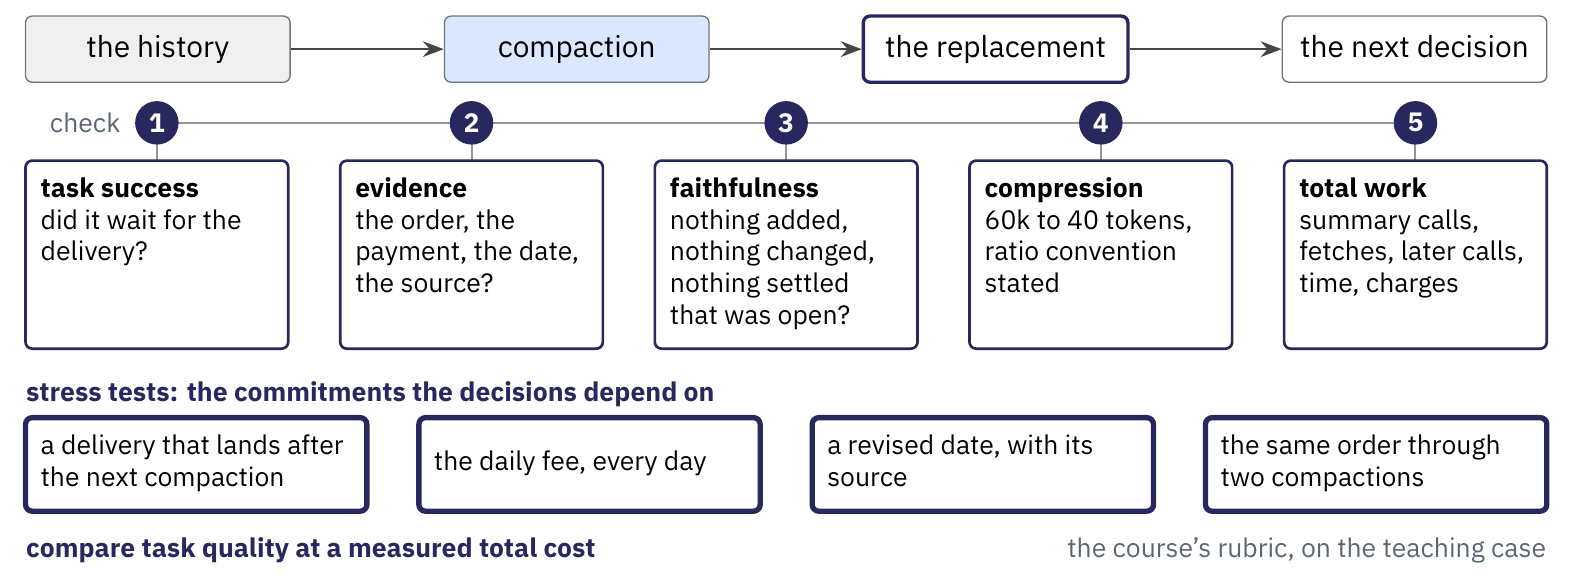
\includegraphics[width=\linewidth]{context/evaluation-6.png}
\caption{Stress tests target what compaction can lose. The figure as it stands after the build's last click.}
\label{fig:evaluation-6}
\end{figure}

\paragraph{The figure, stage by stage.}
\be
\item Check 5, total work: summary calls, fetches, later calls, time, charges. The five checks are reported together, because a compression ratio alone cannot show that a policy serves its task.
\item The stress tests plant the commitments the decisions depend on: 'a delivery that lands after the next compaction', 'the daily fee, every day', 'a revised date, with its source' and 'the same order through two compactions'. The navy line states the rule of the five checks: compare task quality at a measured total cost.
\ee

\begin{takeaway}Each test plants a commitment and checks that it survives compaction.\end{takeaway}

\subsection{Contexts become part of execution state}
\label{sec:it-11-1}

\bi
\item \textbf{Today:} choosing, transforming and evaluating what each call receives.
\item \textbf{Next week:} execution state keeps these contexts for checkpoints, resumption and replay.
\ei

Today we chose, transformed and evaluated what each call receives. Next week keeps these contexts in state: state ownership, run-local and durable state, checkpoint boundaries, resumption and replay. The vending run returns there, because the commitments it carries forward are what a checkpoint must hold.

The lane of steps and checkpoints is schematic, a preview of next week with illustrative counts.

\begin{figure}[htbp]
\centering
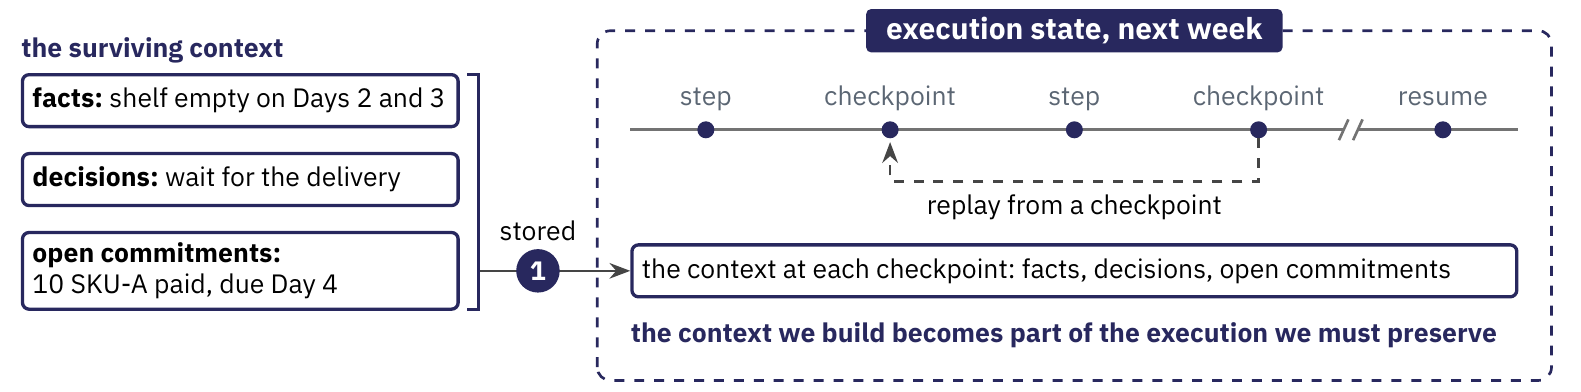
\includegraphics[width=\linewidth]{context/state-bridge-2.png}
\caption{Contexts become part of execution state. The figure as it stands after the build's last click.}
\label{fig:state-bridge-2}
\end{figure}

\paragraph{The figure, stage by stage.}
\be
\item The surviving context: three chips hold ``facts: shelf empty on Days 2 and 3'', ``decisions: wait for the delivery'' and ``open commitments: 10 SKU-A paid, due Day 4''. The dashed ghost ``execution state, next week'' reserves the place where this context goes next.
\item The execution state: the run passes ``step'' and ``checkpoint'' twice, breaks, and goes on at ``resume'', and the dashed arrow marks ``replay from a checkpoint''. A bracket gathers all three chips, and arrow 1, ``stored'', carries them into ``the context at each checkpoint: facts, decisions, open commitments'', so ``the context we build becomes part of the execution we must preserve''.
\ee

\begin{takeaway}A checkpoint must hold the context that the harness has built.\end{takeaway}

\subsection*{Key points}
\bi
\item A policy is judged by the decisions it supports and by the work it costs.
\item Each test plants a commitment and checks that it survives compaction.
\item A checkpoint must hold the context that the harness has built.
\ei
